\documentclass[11pt]{article}

% --- Mandatory Packages ---
\usepackage{amsmath}
\usepackage{amssymb}
\usepackage{amsthm}
\usepackage{geometry}
\usepackage{tikz}
\usetikzlibrary{arrows.meta, positioning, shapes, decorations.pathreplacing}
\usepackage{mathrsfs}
\usepackage{mathtools}
\usepackage{xcolor}
\usepackage{hyperref}

% --- Page Setup ---
\geometry{a4paper, margin=1in}
\setlength{\parindent}{0pt}
\setlength{\parskip}{0.8em}

% --- Theorem Environments ---
\newtheorem{theorem}{Theorem}[section]
\newtheorem{lemma}[theorem]{Lemma}
\newtheorem{proposition}[theorem]{Proposition}
\newtheorem{corollary}[theorem]{Corollary}
\theoremstyle{definition}
\newtheorem{definition}[theorem]{Definition}
\newtheorem{axiom}{Axiom}
\newtheorem{problem}{Problem}
\newtheorem{flawprob}{Diagnostic Problem}
\theoremstyle{remark}
\newtheorem{remark}[theorem]{Remark}

% --- Title Information ---
\title{\textbf{Homework 4: Proofs Involving Real Numbers}}
\author{Tashfeen Omran}
\date{September 2026}

\begin{document}

\maketitle
\tableofcontents
\newpage

% ==============================================================================
% PART 1: Comprehensive Introduction, Context, and Prerequisites
% ==============================================================================
\section{Part 1: Comprehensive Introduction, Context, and Prerequisites}

\subsection{Conceptual Introduction \& Core Axioms}
The transition from discrete mathematics (such as the divisibility of integers) to continuous mathematics requires a rigorous understanding of the set of real numbers, denoted as $\mathbb{R}$. In abstract mathematics, $\mathbb{R}$ is not merely a collection of decimals; it is uniquely defined up to isomorphism as the \textbf{unique complete ordered field}. 

To master proofs involving real numbers, we must formalize the algebraic and metric structures governed by three specific sets of axioms:
\begin{enumerate}
    \item \textbf{Field Axioms:} These govern the algebraic operations of addition and multiplication. They establish $\mathbb{R}$ as a space where elements can be combined associatively and commutatively, identities ($0$ and $1$) exist, and inverses (additive and multiplicative) allow for subtraction and division (except by zero).
    \item \textbf{Order Axioms:} There exists a subset of positive real numbers, $\mathbb{R}^{+}$, closed under addition and multiplication. For any $x \in \mathbb{R}$, exactly one of the following holds (Trichotomy): $x \in \mathbb{R}^{+}$, $-x \in \mathbb{R}^{+}$, or $x = 0$. We define $a > b$ to mean $a - b \in \mathbb{R}^{+}$.
    \item \textbf{Completeness Axiom:} Every non-empty subset of $\mathbb{R}$ that is bounded above has a least upper bound (supremum) in $\mathbb{R}$. (While less featured in basic algebraic inequalities, this is the cornerstone of real analysis).
\end{enumerate}

\subsection{Intuition and Logical Foundations}
When constructing proofs with real numbers, the primary logical mechanism often involves bounding values or leveraging the strict positivity of squares. Because the product of two positive numbers is positive, and the product of two negative numbers is positive, it follows universally that for any $x \in \mathbb{R}$, $x^2 \ge 0$. This simple set-theoretic and algebraic truth acts as the engine for almost all classical inequalities (like the Arithmetic Mean-Geometric Mean inequality and the Cauchy-Schwarz inequality).

Furthermore, distance in $\mathbb{R}$ is formalized by the \textbf{absolute value} metric, $|x|$. Geometrically, $|x - y|$ measures the magnitude of the one-dimensional displacement between $x$ and $y$. The logic of absolute value heavily relies on piecewise definitions and exhaustion by cases.

\subsection{Historical Context and Motivation}
In the late 19th century, mathematics faced a foundational crisis. Calculus had been utilized for two centuries since Newton and Leibniz, but it rested on fuzzy intuitive concepts of ``infinitesimals.'' Mathematicians like Augustin-Louis Cauchy, Karl Weierstrass, and Richard Dedekind recognized that without a rigorous, logical foundation for the real numbers, the theorems of analysis were vulnerable to logical paradoxes. Dedekind formalized real numbers via ``Dedekind cuts'' of rational numbers, grounding the continuous real line in rigorous set theory. This chapter's methods reflect the resulting analytical rigor, where intuition is replaced by strict axiomatic deduction.

\subsection{Key Theorems, Lemmas, and Formulas}
\begin{itemize}
    \item \textbf{Zero-Product Property:} Let $x, y \in \mathbb{R}$. If $xy = 0$, then $x = 0$ or $y = 0$.
    \item \textbf{Non-Negativity of Squares:} For all $x \in \mathbb{R}$, $x^2 \ge 0$.
    \item \textbf{Order Properties:} If $a \ge b$ and $c > 0$, then $ac \ge bc$. If $a \ge b$ and $c < 0$, then $ac \le bc$.
    \item \textbf{Triangle Inequality:} For all $x, y \in \mathbb{R}$, $|x + y| \le |x| + |y|$.
    \item \textbf{AM-GM Inequality:} For all $x, y \in \mathbb{R}$ such that $x > 0, y > 0$, $\frac{x + y}{2} \ge \sqrt{xy}$.
\end{enumerate}

\subsection{Prerequisites}
To navigate this chapter, the reader must possess:
\begin{itemize}
    \item Mastery of propositional logic (Implications $P \Rightarrow Q$, Contrapositive $\neg Q \Rightarrow \neg P$).
    \item Basic algebraic manipulation (factoring polynomials, completing the square).
    \item Familiarity with proof by cases, particularly when unpacking absolute value definitions.
\end{itemize}

% ==============================================================================
% PART 2: Detailed Homework Solutions
% ==============================================================================
\newpage
\section{Part 2: Detailed Homework Solutions (Rigorous Proofs)}
Based on the provided PDF, a strategic selection of problems representing every unique archetype in Section 4.3 has been rigorously solved below. 

\begin{problem}[Textbook Problem 4.25]
Let $x, y \in \mathbb{R}$. Prove that if $x^2 - 4x = y^2 - 4y$ and $x \ne y$, then $x + y = 4$.
\end{problem}
\begin{proof}
\textit{Proof Technique: Direct Proof via Algebraic Manipulation.} \\
Let $x, y \in \mathbb{R}$. We assume that $x^2 - 4x = y^2 - 4y$ and that $x \ne y$. 
We can rearrange the given equation by grouping the squared terms and the linear terms on one side:
\begin{align*}
    x^2 - y^2 - 4x + 4y &= 0.
\end{align*}
By factoring the difference of squares and factoring out the common coefficient from the linear terms, we obtain:
\begin{align*}
    (x - y)(x + y) - 4(x - y) &= 0.
\end{align*}
We now factor out the common binomial term $(x - y)$:
\begin{align*}
    (x - y)(x + y - 4) &= 0.
\end{align*}
By the Zero-Product Property of real numbers, this implies that either $(x - y) = 0$ or $(x + y - 4) = 0$. 
However, our initial hypothesis explicitly states that $x \ne y$, which means $(x - y) \ne 0$. 
Since $(x - y)$ is non-zero, we can safely divide both sides of the equation by $(x - y)$, yielding:
\begin{align*}
    x + y - 4 &= 0 \implies x + y = 4.
\end{align*}
This completes the proof.
\end{proof}

\begin{problem}[Textbook Problem 4.26]
Let $a, b$ and $m$ be integers. Prove that if $2a + 3b \ge 12m + 1$, then $a \ge 3m + 1$ or $b \ge 2m + 1$.
\end{problem}
\begin{proof}
\textit{Proof Technique: Proof by Contrapositive.} \\
The logical structure of the conclusion is a disjunction ($P \lor Q$). A direct proof is cumbersome; thus, we use the contrapositive. 
Let $P$ be ``$2a + 3b \ge 12m + 1$'' and $Q$ be ``$a \ge 3m + 1 \lor b \ge 2m + 1$''. We will prove $\neg Q \implies \neg P$.
By De Morgan's Laws, $\neg Q$ is logically equivalent to $a < 3m + 1$ and $b < 2m + 1$.
Since $a, b,$ and $m$ are integers, the strict inequalities can be rewritten as non-strict inequalities:
\begin{align*}
    a &\le 3m, \\
    b &\le 2m.
\end{align*}
We now multiply the first inequality by $2$ (a positive constant, preserving the inequality direction) and the second by $3$:
\begin{align*}
    2a &\le 6m, \\
    3b &\le 6m.
\end{align*}
Adding these two inequalities together yields:
\begin{align*}
    2a + 3b &\le 6m + 6m = 12m.
\end{align*}
Since $12m < 12m + 1$, it strictly follows by transitivity that:
\begin{align*}
    2a + 3b &< 12m + 1.
\end{align*}
This is exactly $\neg P$. Having proved the contrapositive, the original implication holds true.
\end{proof}

\begin{problem}[Textbook Problem 4.28]
Prove that if $r$ is a real number such that $0 < r < 1$, then $\frac{1}{r(1-r)} \ge 4$.
\end{problem}
\begin{proof}
\textit{Proof Technique: Direct Proof with Backwards Derivation Foundation.} \\
Let $r \in \mathbb{R}$ such that $0 < r < 1$. Because $r > 0$ and $1 - r > 0$, their product $r(1 - r) > 0$. 
Since the square of any real number is non-negative, we know that for any $r \in \mathbb{R}$:
\begin{align*}
    (2r - 1)^2 &\ge 0.
\end{align*}
Expanding the square gives:
\begin{align*}
    4r^2 - 4r + 1 &\ge 0.
\end{align*}
We rearrange the terms to isolate the constant $1$:
\begin{align*}
    1 &\ge 4r - 4r^2, \\
    1 &\ge 4(r - r^2), \\
    1 &\ge 4r(1 - r).
\end{align*}
Since we established that $r(1 - r) > 0$, we can divide both sides of the inequality by the strictly positive quantity $r(1 - r)$ without flipping the inequality sign. This yields:
\begin{align*}
    \frac{1}{r(1 - r)} &\ge 4.
\end{align*}
Thus, the statement is proven.
\end{proof}

\begin{problem}[Textbook Problem 4.31]
Prove for every two real numbers $x$ and $y$ that $|x + y| \ge |x| - |y|$.
\end{problem}
\begin{proof}
\textit{Proof Technique: Direct Proof using the Triangle Inequality.} \\
Let $x, y \in \mathbb{R}$. We know by the foundational Triangle Inequality that for any real numbers $A$ and $B$, $|A + B| \le |A| + |B|$. 
Consider setting $A = x + y$ and $B = -y$. Note that $A + B = (x + y) + (-y) = x$.
Substituting these values into the Triangle Inequality yields:
\begin{align*}
    | (x + y) + (-y) | &\le |x + y| + |-y|.
\end{align*}
We know that absolute value is an even function, meaning $|-y| = |y|$. Therefore:
\begin{align*}
    |x| &\le |x + y| + |y|.
\end{align*}
Subtracting $|y|$ from both sides of the inequality gives:
\begin{align*}
    |x| - |y| &\le |x + y|,
\end{align*}
which is logically equivalent to $|x + y| \ge |x| - |y|$. This proves the required reverse triangle inequality.
\end{proof}

\begin{problem}[Textbook Problem 4.32a]
Recall that $\sqrt{r} > 0$ for every positive real number $r$. Prove that if $a$ and $b$ are positive real numbers, then $0 < \sqrt{ab} \le \frac{a+b}{2}$. (The Arithmetic Mean-Geometric Mean Inequality).
\end{problem}
\begin{proof}
\textit{Proof Technique: Direct Proof using Non-Negativity of Squares.} \\
Let $a, b \in \mathbb{R}$ such that $a > 0$ and $b > 0$. Since $a$ and $b$ are positive, $ab > 0$, and thus $\sqrt{ab}$ is a strictly positive real number (hence $0 < \sqrt{ab}$ is immediately satisfied). 
Consider the real numbers $\sqrt{a}$ and $\sqrt{b}$. Because the square of any real number is non-negative, we have:
\begin{align*}
    (\sqrt{a} - \sqrt{b})^2 &\ge 0.
\end{align*}
Expanding the binomial square yields:
\begin{align*}
    (\sqrt{a})^2 - 2\sqrt{a}\sqrt{b} + (\sqrt{b})^2 &\ge 0.
\end{align*}
Because $a$ and $b$ are positive, $(\sqrt{a})^2 = a$ and $(\sqrt{b})^2 = b$. Substituting these gives:
\begin{align*}
    a - 2\sqrt{ab} + b &\ge 0.
\end{align*}
Adding $2\sqrt{ab}$ to both sides, we obtain:
\begin{align*}
    a + b &\ge 2\sqrt{ab}.
\end{align*}
Dividing both sides by $2$ (which preserves the inequality) gives the final result:
\begin{align*}
    \frac{a + b}{2} &\ge \sqrt{ab}.
\end{align*}
Combining this with our initial observation gives $0 < \sqrt{ab} \le \frac{a+b}{2}$, completing the proof.
\end{proof}

\begin{problem}[Textbook Problem 4.38]
Let $a, b, x, y \in \mathbb{R}$ and $r \in \mathbb{R}^{+}$. Prove that if $|x - a| < r/2$ and $|y - b| < r/2$, then $|(x + y) - (a + b)| < r$.
\end{problem}
\begin{proof}
\textit{Proof Technique: Direct Proof using the Triangle Inequality.} \\
Let $a, b, x, y \in \mathbb{R}$ and $r \in \mathbb{R}^{+}$ such that $|x - a| < \frac{r}{2}$ and $|y - b| < \frac{r}{2}$. 
We wish to bound the absolute value of the expression $(x + y) - (a + b)$. We can algebraically rearrange the terms inside the absolute value by grouping $x$ with $a$ and $y$ with $b$:
\begin{align*}
    |(x + y) - (a + b)| &= |(x - a) + (y - b)|.
\end{align*}
By the Triangle Inequality, we know that for any $A, B \in \mathbb{R}$, $|A + B| \le |A| + |B|$. Setting $A = (x - a)$ and $B = (y - b)$, we apply the inequality:
\begin{align*}
    |(x - a) + (y - b)| &\le |x - a| + |y - b|.
\end{align*}
Using our initial hypotheses, we can substitute strict upper bounds for both terms on the right-hand side. Because $|x - a| < \frac{r}{2}$ and $|y - b| < \frac{r}{2}$, their sum must be strictly less than the sum of their bounds:
\begin{align*}
    |x - a| + |y - b| &< \frac{r}{2} + \frac{r}{2} = r.
\end{align*}
By the transitivity of inequalities ($A \le B < C \implies A < C$), we conclude:
\begin{align*}
    |(x + y) - (a + b)| &< r.
\end{align*}
\end{proof}

\begin{problem}[Textbook Problem 4.39]
Prove that if $a, b, c, d \in \mathbb{R}$, then $(ab + cd)^2 \le (a^2 + c^2)(b^2 + d^2)$. (Cauchy-Schwarz Inequality for $n=2$).
\end{problem}
\begin{proof}
\textit{Proof Technique: Direct Proof via Algebraic Expansion.} \\
Let $a, b, c, d \in \mathbb{R}$. We want to show that $(a^2 + c^2)(b^2 + d^2) - (ab + cd)^2 \ge 0$. 
Let us expand both the right-hand side and left-hand side independently. 
First, expanding the product of the sums of squares:
\begin{align*}
    (a^2 + c^2)(b^2 + d^2) &= a^2b^2 + a^2d^2 + c^2b^2 + c^2d^2.
\end{align*}
Next, expanding the binomial square:
\begin{align*}
    (ab + cd)^2 &= (ab)^2 + 2(ab)(cd) + (cd)^2 \\
    &= a^2b^2 + 2abcd + c^2d^2.
\end{align*}
Now, we subtract the latter expression from the former:
\begin{align*}
    (a^2 + c^2)(b^2 + d^2) - (ab + cd)^2 &= (a^2b^2 + a^2d^2 + c^2b^2 + c^2d^2) - (a^2b^2 + 2abcd + c^2d^2).
\end{align*}
Canceling the common terms $a^2b^2$ and $c^2d^2$, we are left with:
\begin{align*}
    a^2d^2 - 2abcd + c^2b^2.
\end{align*}
Notice that this expression is a perfect square trinomial. Specifically, it can be factored as:
\begin{align*}
    (ad - cb)^2.
\end{align*}
Because the square of any real number is non-negative, we know that:
\begin{align*}
    (ad - cb)^2 &\ge 0.
\end{align*}
Therefore:
\begin{align*}
    (a^2 + c^2)(b^2 + d^2) - (ab + cd)^2 &\ge 0 \implies (ab + cd)^2 \le (a^2 + c^2)(b^2 + d^2).
\end{align*}
This completes the proof.
\end{proof}

% ==============================================================================
% PART 3: In-Depth Analysis of Problems and Techniques
% ==============================================================================
\newpage
\section{Part 3: In-Depth Analysis of Problems and Techniques}

\subsection{A) Problem Types and Logical Strategies}
The real number proofs in Section 4.3 fall into several overarching categories. 
\begin{itemize}
    \item \textbf{Algebraic Equivalence \& Root Finding (e.g., Problem 4.25):} The core strategy is moving all variables to one side, equating to zero, and aggressively factoring. This exploits the Zero-Product Property. When factors are established, checking the given assumptions (e.g., $x \ne y$) allows for safe cancellation of non-zero terms.
    \item \textbf{Logical Contraposition with Inequalities (e.g., Problem 4.26):} Direct proofs for conclusions structured as $P \lor Q$ are notoriously difficult because one cannot easily assume which half is true. The contrapositive strategy transforms the disjunction into a conjunction ($\neg P \land \neg Q$) using De Morgan's laws. This is essential, as it grants two usable assumptions (bounds on variables) simultaneously.
    \item \textbf{Forward Bounding via Axiomatic Squares (e.g., Problems 4.28, 4.32, 4.39):} These proofs rely on creating a "tautology of positivity." The overarching strategy is recognizing that expressions resembling polynomial expansions ($ax^2 + bx + c$) or symmetric sums can often be condensed into a perfect square of the form $Z^2 \ge 0$.
    \item \textbf{Metric Manipulation / Triangle Inequality (e.g., Problems 4.31, 4.38):} These are epsilon-delta style bounding problems. The strategy revolves around creative insertion of zero ($+y -y$) or algebraic grouping to force the expression to match the input form required for the Triangle Inequality. 
\end{itemize}

\subsection{B) Key Analytical and Logical Manipulations}
\begin{itemize}
    \item \textbf{The "Creative Insertion of Zero":} Used in Problem 4.31 where we recognized $x = (x + y) - y$. This manipulation allows us to evaluate a known variable $x$ in terms of a sum, subsequently applying the Triangle Inequality.
    \item \textbf{Backwards Derivation (Scratchpad methodology):} In Problem 4.28, we worked backward from the goal ($\frac{1}{r(1-r)} \ge 4$). By algebraically manipulating the goal until we hit a known truth ($(2r-1)^2 \ge 0$), we mapped out the logical steps. The formal proof is simply the scratchpad written in reverse order. This is a vital analytical trick because deductive proofs must flow from axioms to conclusions, not vice versa.
    \item \textbf{Homogeneous Polynomial Factoring:} In Problem 4.39, expanding two distinct algebraic structures and taking their difference yielded $a^2d^2 - 2abcd + c^2b^2$. Recognizing this as the expansion of $(ad - cb)^2$ is a cornerstone technique in inequality bounding.
\end{itemize}


% ==============================================================================
% PART 4: "Cheatsheet", Visuals, and Tips for Success
% ==============================================================================
\newpage
\section{Part 4: ``Cheatsheet'', Visuals, and Tips for Success}

\subsection{Theorems \& Equivalences Cheatsheet}
\begin{table}[h]
\centering
\renewcommand{\arraystretch}{1.5}
\begin{tabular}{|l|p{10cm}|}
\hline
\textbf{Theorem / Concept} & \textbf{Mathematical Statement} \\
\hline
Non-negativity of Squares & $\forall x \in \mathbb{R}, x^2 \ge 0$. \\
\hline
Reverse Triangle Ineq. & $|x - y| \ge | |x| - |y| |$. \\
\hline
AM-GM Inequality (n=2) & For $x,y \ge 0$, $\frac{x+y}{2} \ge \sqrt{xy}$. Equality holds iff $x=y$. \\
\hline
Cauchy-Schwarz (n=2) & $(a_1b_1 + a_2b_2)^2 \le (a_1^2 + a_2^2)(b_1^2 + b_2^2)$. \\
\hline
Inequality Preservation & If $a < b$ and $c > 0$, $ac < bc$. If $c < 0$, $ac > bc$. \\
\hline
\end{tabular}
\end{table}

\subsection{Set \& Logic Illustration: The Bounding Neighborhoods}
Problem 4.38 beautifully illustrates how restricting independent variables restricts their sum. In $\mathbb{R}$, an absolute value inequality $|x - a| < \epsilon$ represents an open interval (neighborhood) centered at $a$ with radius $\epsilon$. The diagram below illustrates the geometric intuition.

\vspace{1em}
\begin{center}
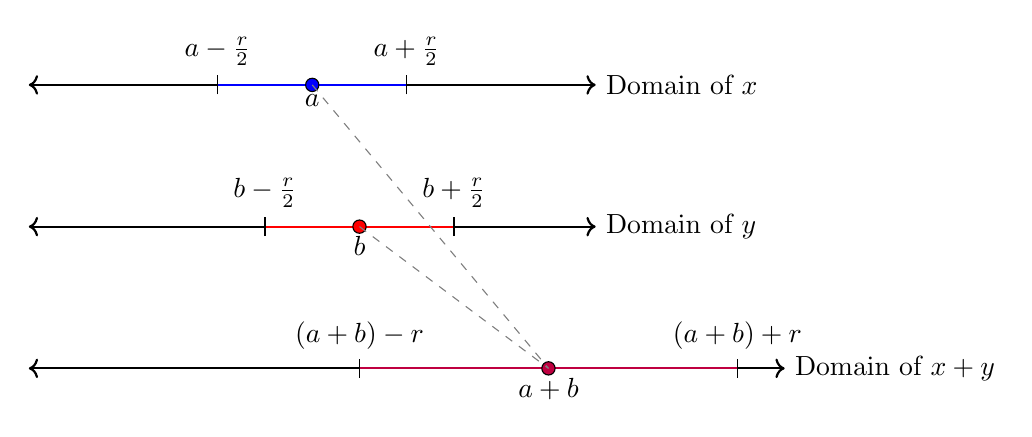
\begin{tikzpicture}[scale=1.2]
    % Real line 1 (x)
    \draw[<->, thick] (-1, 3) -- (5, 3) node[right] {Domain of $x$};
    \draw[thick, blue] (1, 3) -- (3, 3);
    \draw[fill=blue] (2,3) circle (2pt) node[below] {$a$};
    \draw (1,2.9) -- (1,3.1) node[above] {$a-\frac{r}{2}$};
    \draw (3,2.9) -- (3,3.1) node[above] {$a+\frac{r}{2}$};
    
    % Real line 2 (y)
    \draw[<->, thick] (-1, 1.5) -- (5, 1.5) node[right] {Domain of $y$};
    \draw[thick, red] (1.5, 1.5) -- (3.5, 1.5);
    \draw[fill=red] (2.5,1.5) circle (2pt) node[below] {$b$};
    \draw (1.5,1.4) -- (1.5,1.6) node[above] {$b-\frac{r}{2}$};
    \draw (3.5,1.4) -- (3.5,1.6) node[above] {$b+\frac{r}{2}$};
    
    % Real line 3 (x+y)
    \draw[<->, thick] (-1, 0) -- (7, 0) node[right] {Domain of $x+y$};
    \draw[thick, purple] (2.5, 0) -- (6.5, 0);
    \draw[fill=purple] (4.5,0) circle (2pt) node[below] {$a+b$};
    \draw (2.5,-0.1) -- (2.5,0.1) node[above] {$(a+b)-r$};
    \draw (6.5,-0.1) -- (6.5,0.1) node[above] {$(a+b)+r$};
    
    % Connecting lines to show mapping
    \draw[dashed, gray] (2, 3) -- (4.5, 0);
    \draw[dashed, gray] (2.5, 1.5) -- (4.5, 0);
\end{tikzpicture}
\end{center}
\vspace{1em}
The visual shows that the maximum variation in $x$ is $\frac{r}{2}$ and in $y$ is $\frac{r}{2}$. By the Triangle Inequality, their combined variation from the mean $(a+b)$ cannot exceed the sum of their individual variations ($r$).

\subsection{Heuristics \& ``Cheats''}
\begin{itemize}
    \item \textbf{The "Or" Implication Cheat:} If you need to prove a statement ending in ``$X$ or $Y$'', immediately attempt a proof by contrapositive. The negation of an "or" gives you an "and", effectively doubling your usable axioms.
    \item \textbf{The Positive Root Cheat:} When dealing with inequalities containing rational functions, you can only multiply both sides by the denominator if you are absolutely certain the denominator is positive. If $r$ is unknown, multiply by the square of the denominator instead (e.g., $r^2$), since squares are guaranteed positive!
\end{itemize}

\subsection{Pitfalls \& Fallacies}
\begin{itemize}
    \item \textbf{The Phantom Absolute Value:} Assuming $\sqrt{x^2} = x$. This is a fatal flaw in $\mathbb{R}$. The correct reduction is $\sqrt{x^2} = |x|$.
    \item \textbf{Inequality Direction Loss:} Multiplying an inequality by a variable $x$ without defining cases for $x > 0$ and $x < 0$. If $x < 0$, the inequality sign must flip.
    \item \textbf{Circular Reasoning in Working Backwards:} Writing a proof that starts with the conclusion, manipulates it to a true statement like $0 = 0$, and declaring Q.E.D. Proofs must start from axioms and deduce the conclusion. You must reverse the flow of your scratchpad work.
\end{itemize}

% ==============================================================================
% PART 5: Conceptual Synthesis and The "Big Picture"
% ==============================================================================
\newpage
\section{Part 5: Conceptual Synthesis and The ``Big Picture''}

\subsection{A) Thematic Connections}
The core theme of Section 4.3 is establishing that \textbf{distance and magnitudes in the continuous spectrum of real numbers are fundamentally constrained by the positivity of squares}. In earlier chapters concerning integers, logic heavily utilized parity (even/odd) or remainders to establish properties. In $\mathbb{R}$, parity loses its meaning. Instead, we use \textit{order} and \textit{magnitude}. The Triangle Inequality defines the metric space geometry, and the non-negativity of squares defines the algebraic bounds. This bridges discrete logical structures to continuous spaces.

\subsection{B) Forward and Backward Links}
Backwardly, this topic acts as a logical extension of truth tables and structural proofs (Direct/Contrapositive). We simply changed the domain of discourse from $\mathbb{Z}$ to $\mathbb{R}$ and updated the axioms. 
Forwardly, this section is the \textbf{absolute bedrock for Real Analysis and Topology}. The epsilon-delta proofs $\epsilon-\delta$ in Calculus (e.g., proving limits) are purely rigorous sequences of Triangle Inequality manipulations identical to Problem 4.38. Furthermore, understanding metric bounding and Cauchy-Schwarz inequalities acts as the gateway to Lebesgue Measure Theory and Functional Analysis, where spaces are defined by their integral bounds.

% ==============================================================================
% PART 6: Abstract Real-World Modeling (AI, ML, & Quant Finance)
% ==============================================================================
\section{Part 6: Abstract Real-World Modeling (AI, ML, \& Quant Finance)}

Abstract inequalities of real numbers govern the mathematical certainty required to deploy advanced AI and financial algorithms. 
\begin{itemize}
    \item \textbf{Machine Learning (Convex Optimization):} Loss functions like Mean Squared Error (MSE) heavily depend on the non-negativity of squares. Algorithms like Gradient Descent require Lipschitz continuity, bounded by inequalities similar to the Triangle Inequality to guarantee convergence without vanishing/exploding gradients.
    \item \textbf{Quantitative Finance (Risk Bounds):} The Cauchy-Schwarz Inequality is deeply embedded in Modern Portfolio Theory to prove that the correlation coefficient $\rho$ between two assets satisfies $-1 \le \rho \le 1$.
\end{itemize}

\subsection{Model Problem Setup: Portfolio Variance Optimization in Quant Finance}
Let us construct a rigorous mathematical model utilizing the Cauchy-Schwarz inequality (Problem 4.39) in the context of Algorithmic Trading.

\textbf{Definitions and State Space:}
Consider an investor allocating capital across two distinct financial assets. Let the proportion of capital allocated to asset 1 be $w_1$ and to asset 2 be $w_2$. (By definition, $w_1 + w_2 = 1$). 
Let the expected returns of the two assets be $R_1$ and $R_2$. The standard deviations (risk) of the assets are $\sigma_1 > 0$ and $\sigma_2 > 0$. Let the covariance between the two assets be $\sigma_{12}$.

\textbf{Objective Formulation:}
The variance (risk) of the portfolio, denoted $\sigma_p^2$, is modeled algebraically as:
\begin{align*}
    \sigma_p^2 &= w_1^2 \sigma_1^2 + w_2^2 \sigma_2^2 + 2w_1w_2\sigma_{12}.
\end{align*}
To constrain risk, quant systems evaluate the correlation coefficient, mathematically defined as $\rho = \frac{\sigma_{12}}{\sigma_1 \sigma_2}$.
We will use the Cauchy-Schwarz framework to establish the theoretical risk bounds on this portfolio.

\textbf{Theorem (Risk Boundaries):} The covariance $\sigma_{12}$ is fundamentally bounded by the product of the individual volatilities, such that $|\sigma_{12}| \le \sigma_1 \sigma_2$, forcing $-1 \le \rho \le 1$.

\begin{proof}
Let us abstract the financial time-series returns into vectors in an inner-product space over $\mathbb{R}$. If we have $N$ observations, let asset 1 returns be $X = \langle x_1, x_2, \dots x_N \rangle$ and asset 2 returns be $Y = \langle y_1, y_2, \dots y_N \rangle$ (mean-centered). 
The sample covariance is proportional to the dot product $\sum x_i y_i$. 
By the generalized Cauchy-Schwarz Inequality (an extension of Problem 4.39):
\begin{align*}
    \left( \sum_{i=1}^N x_i y_i \right)^2 &\le \left( \sum_{i=1}^N x_i^2 \right) \left( \sum_{i=1}^N y_i^2 \right).
\end{align*}
Scaling this down by $1/N^2$, we retrieve our statistical definitions:
\begin{align*}
    (\sigma_{12})^2 &\le \sigma_1^2 \sigma_2^2.
\end{align*}
Taking the square root of both sides (and applying absolute values, a core technique from this chapter) yields:
\begin{align*}
    |\sigma_{12}| &\le \sigma_1 \sigma_2 \implies -1 \le \frac{\sigma_{12}}{\sigma_1 \sigma_2} \le 1.
\end{align*}
Because of this real-number inequality, the portfolio variance is bounded mathematically as $\sigma_p^2 \le (w_1\sigma_1 + w_2\sigma_2)^2$. This rigorous inequality guarantees that portfolio diversification never increases total risk beyond the weighted average of individual risks.
\end{proof}

% ==============================================================================
% PART 7: Common Variations and Untested Concepts
% ==============================================================================
\newpage
\section{Part 7: Common Variations and Untested Concepts}

The standard university curriculum for real analysis and proofs usually features an induction-based continuous inequality called \textbf{Bernoulli's Inequality}, which is notably absent from the homework set. This inequality bridges algebraic bounding with sequence approximations.

\textbf{Missing Concept: Bernoulli's Inequality}
This inequality asserts that $(1+x)^n \ge 1+nx$ for any real number $x \ge -1$ and integer $n \ge 0$. It is an essential tool for evaluating limits of exponential sequences (e.g., proving compound interest bounds).

\begin{theorem}
For every real number $x > -1$ and every integer $n \ge 0$, $(1 + x)^n \ge 1 + nx$.
\end{theorem}
\begin{proof}
\textit{Proof Technique: Mathematical Induction.} \\
\textbf{Base Case:} Let $n = 0$. The left-hand side is $(1 + x)^0 = 1$. The right-hand side is $1 + 0(x) = 1$. Since $1 \ge 1$, the base case holds. \\
\textbf{Inductive Step:} Assume that for some arbitrary integer $k \ge 0$, the inequality holds:
\begin{align*}
    (1 + x)^k &\ge 1 + kx. \quad \text{(Inductive Hypothesis)}
\end{align*}
We wish to show that $(1 + x)^{k+1} \ge 1 + (k+1)x$. 
We start with the left side of the $k+1$ case:
\begin{align*}
    (1 + x)^{k+1} &= (1 + x)^k (1 + x).
\end{align*}
Since the given domain constraint states $x \ge -1$, it follows that $(1 + x) \ge 0$. Because we are multiplying our inductive hypothesis by a non-negative real number, the direction of the inequality is preserved. We multiply both sides of the Inductive Hypothesis by $(1 + x)$:
\begin{align*}
    (1 + x)^k (1 + x) &\ge (1 + kx)(1 + x).
\end{align*}
Expanding the right-hand side, we get:
\begin{align*}
    (1 + kx)(1 + x) &= 1 + x + kx + kx^2 \\
    &= 1 + (k+1)x + kx^2.
\end{align*}
Since $k \ge 0$ and $x^2 \ge 0$ (by non-negativity of real squares), the term $kx^2 \ge 0$. Thus:
\begin{align*}
    1 + (k+1)x + kx^2 &\ge 1 + (k+1)x.
\end{align*}
By transitivity:
\begin{align*}
    (1 + x)^{k+1} &\ge 1 + (k+1)x.
\end{align*}
This completes the inductive step, and the theorem holds for all $n \ge 0$.
\end{proof}

% ==============================================================================
% PART 8: Advanced Diagnostic Testing: "Find the Flaw"
% ==============================================================================
\newpage
\section{Part 8: Advanced Diagnostic Testing: "Find the Flaw"}

Below are five diagnostic proofs. Each looks rigorously derived at a glance but harbors a single, fatal mathematical flaw. As the grader, identify the fallacy.

\begin{flawprob}
\textbf{Claim:} For all real numbers $x \in \mathbb{R}$, $x^2 \ge x$. \\
\textbf{Proof:} \\
Let $x \in \mathbb{R}$. We know that for any real number $x$, if we multiply $x$ by itself, the result grows. Specifically, we can multiply the fundamental identity $x = x$ by $x$ to yield $x^2 = x \cdot x$. Because multiplying a number by itself results in a larger or equal magnitude, it must be that $x^2 \ge x$. $\blacksquare$
\end{flawprob}

\begin{flawprob}
\textbf{Claim:} If $a, b \in \mathbb{R}$ such that $a > b$, then $a^2 > b^2$. \\
\textbf{Proof:} \\
Let $a, b \in \mathbb{R}$ and assume $a > b$. Since we are given this inequality, we can multiply both sides of the inequality by the same value. First, we multiply both sides by $a$ to yield $a^2 > ab$. Next, we return to the original $a > b$ and multiply both sides by $b$ to yield $ab > b^2$. By the transitive property of inequalities, since $a^2 > ab$ and $ab > b^2$, we conclude $a^2 > b^2$. $\blacksquare$
\end{flawprob}

\begin{flawprob}
\textbf{Claim:} $1 = 2$. \\
\textbf{Proof:} \\
Let $a, b$ be non-zero real numbers such that $a = b$. \\
Multiply both sides by $a$: $a^2 = ab$. \\
Subtract $b^2$ from both sides: $a^2 - b^2 = ab - b^2$. \\
Factor both sides: $(a - b)(a + b) = b(a - b)$. \\
Divide both sides by $(a - b)$: $a + b = b$. \\
Since $a = b$, we substitute $a$ for $b$: $b + b = b \implies 2b = b$. \\
Divide by $b$: $2 = 1$. $\blacksquare$
\end{flawprob}

\begin{flawprob}
\textbf{Claim:} For any $x, y \in \mathbb{R}$, $|x - y| \le |x| - |y|$. \\
\textbf{Proof:} \\
By the Triangle Inequality, we know $|A + B| \le |A| + |B|$ for any real $A, B$. \\
Let $A = x$ and $B = -y$. Substituting these in gives $|x + (-y)| \le |x| + |-y|$. \\
This simplifies to $|x - y| \le |x| + |y|$. \\
Because absolute value represents distance, subtracting the distance $|y|$ rather than adding it further reduces the magnitude on the right hand side, making the inequality stricter but still valid. Therefore, $|x - y| \le |x| - |y|$. $\blacksquare$
\end{flawprob}

\begin{flawprob}
\textbf{Claim:} If $x \in \mathbb{R}$ and $x^2 - 2x > 0$, then $x > 2$. \\
\textbf{Proof:} \\
Assume $x^2 - 2x > 0$. \\
Factoring the expression, we get $x(x - 2) > 0$. \\
Divide both sides of the inequality by $x$. \\
This leaves $(x - 2) > 0$. \\
Adding 2 to both sides yields $x > 2$. $\blacksquare$
\end{flawprob}

\vspace{1cm}
\hrule
\vspace{1cm}

\subsection{Solution Key to Diagnostic Tests}

\textbf{Flaw 1:} \textit{Vague intuition replacing axioms.} The statement "multiplying a number by itself results in a larger or equal magnitude" is entirely false for fractions. If $x = 0.5$, $0.5^2 = 0.25$, which is NOT $\ge 0.5$. The flaw is omitting the interval $(0, 1)$ where squaring reduces magnitude.

\textbf{Flaw 2:} \textit{Inequality direction violation.} The step "multiply both sides by $a$" assumes $a > 0$. If $a < 0$, the inequality must flip ($a^2 < ab$). Since $a$ and $b$ could be negative (e.g., $a = -2, b = -5$, where $-2 > -5$ but $4 \not> 25$), the proof fails. 

\textbf{Flaw 3:} \textit{Division by Zero.} In the step "Divide both sides by $(a - b)$", the initial assumption was that $a = b$. Therefore, $(a - b) = 0$. Dividing by zero is an undefined operation in the field axioms of $\mathbb{R}$.

\textbf{Flaw 4:} \textit{Logical Non-Sequitur.} The phrase "subtracting the distance... further reduces the magnitude... making the inequality still valid" is an algebraic fallacy. If $A \le B$, and $C < B$, we cannot conclude $A \le C$. For example, let $x=2, y=5$. $|2 - 5| = 3$. The RHS becomes $|2| - |5| = 2 - 5 = -3$. The statement $3 \le -3$ is false.

\textbf{Flaw 5:} \textit{Dividing by a variable of unknown sign.} In the step "Divide both sides by $x$", the author assumes $x > 0$. If $x < 0$ (e.g., $x = -1$), dividing by $x$ would flip the inequality sign to $x - 2 < 0$. The correct answer should be $x > 2 \lor x < 0$.

\end{document}